\documentclass[12pt]{article}

\usepackage[margin=1in]{geometry}
\usepackage[spanish]{babel}
\usepackage{amsmath}
\usepackage{amssymb}
\usepackage{caption}
\usepackage{subcaption}
\usepackage{graphicx}
\graphicspath{{./imagenes/}}

\newcommand{\dint}{\delta_{\text{int}}}
\newcommand{\dext}{\delta_{\text{ext}}}
\newcommand{\estado}{(id, s, vv, vc, pa, \sigma)}
\newcommand{\R}{\mathbb{R}}
\newcommand{\N}{\mathbb{N}}

\title{Juego de la Vida\\
\large~Trabajo práctico para Simulación}
\author{D'Autilio Joel, Rossi Pablo}
\date{}

\begin{document}
\maketitle


\section{El Juego de la Vida de Conway}


Los autómatas celulares son sistemas en los que autómatas simples están conectados localmente con sus autómatas vecinos. Cada uno de estos autómatas se denomina célula y tiene la capacidad de generar una salida basada en múltiples entradas, modificando su estado mediante una función de transición. Por lo general, en los autómatas celulares, el estado de una célula en una generación dada se determina únicamente por los estados de las células vecinas y su propio estado en la generación anterior.

El juego de la vida es un autómata celular diseñado por John Horton Conway en 1970. El universo del Juego de la Vida consiste en una cuadrícula bidimensional compuesta por células individuales que pueden estar en dos estados: vivas o muertas. Cada célula interactúa con sus ocho vecinos más cercanos (arriba, abajo, izquierda, derecha y en diagonal). La evolución de las células ocurre en generaciones discretas, donde el estado de cada célula en una generación se determina por las reglas establecidas. Las reglas del Juego de la Vida de Conway son las siguientes: 

\begin{itemize}
  \item Si una célula está viva, puede seguir viva en la siguiente generación si tiene exactamente dos o tres vecinos vivos. 
  \item Si una célula está viva y tiene menos de dos o más de tres vecinos vivos, morirá en la siguiente generación debido a la soledad o la superpoblación.
  \item Si una célula está muerta, puede ``nacer'' en la siguiente generación si tiene exactamente tres vecinos vivos.
\end{itemize}

Si bien estas son las reglas originales propuestas por Conway, existen variaciones que se expresan comúnmente en formato X/Y, donde X e Y son enteros. La parte X representa las reglas de nacimiento, mientras que la parte Y representa las reglas de supervivencia. Por ejemplo, la regla 23/36 indica que una célula nacerá si tiene 2 o 3 vecinos vivos y sobrevivirá si tiene exactamente 3 o 6 vecinos vivos. En el caso del Juego de la Vida propuesto por Conway, las reglas son 3/23. En la figura~\ref{img:ej1} se muestra una posible secuencia con estas últimas reglas.

\begin{figure}
  \centering
  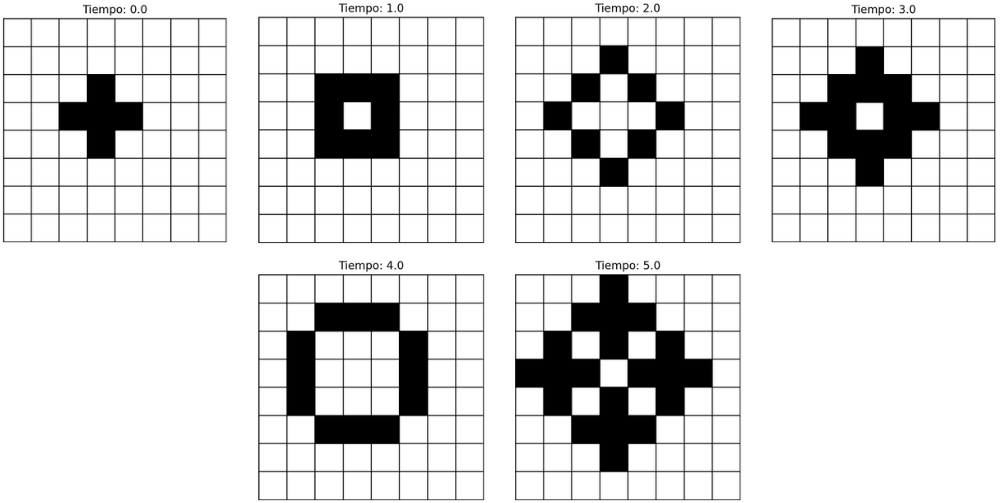
\includegraphics[width=0.8\textwidth]{imagenes/ej1}
  \caption{Una secuencia de estados del juego de la vida con las reglas de Conway (las casillas en negro representan células vivas).}\label{img:ej1}
\end{figure}

A medida que las generaciones avanzan, las células interactúan entre sí, creando patrones en constante cambio. Algunos patrones permanecen estables y estáticos, mientras que otros pueden moverse, girar o incluso replicarse.


\section{Especificación DEVS}


\subsection{Idea intuitiva}


El modelo DEVS que representa al juego de la vida es un acoplado de células que se comunican entre sí. Cada célula tiene un estado que puede ser vivo o muerto, y se actualiza en cada paso de la simulación. Las células se comunican con sus vecinas para conocer sus estados y así poder calcular el suyo.

Llamese $I$ al tiempo entre estados del juego. Queremos que cada $I$ segundos cada célula comunique su nuevo estado y se guarde el tablero. Para esto, siguen un ciclo de dos pasos que llamaremos \textit{Comunicar} y \textit{Actualizar} (fig.~\ref{img:timeline}).

\begin{figure}[ht]
  \centering
  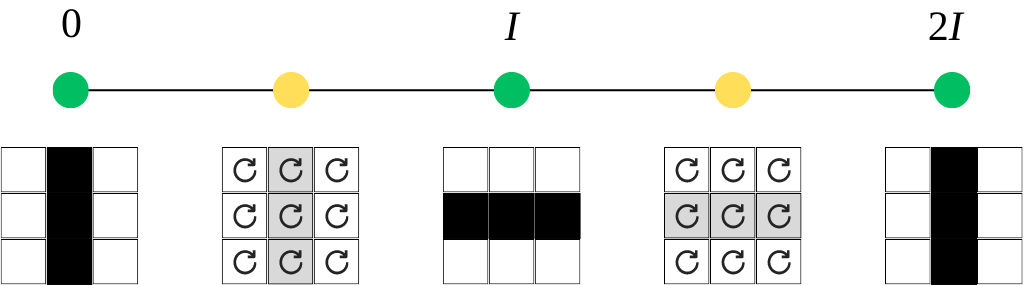
\includegraphics[width=0.8\textwidth]{imagenes/timeline}
  \caption{Ciclo de comunicación y actualización de una célula. En los puntos verdes, la célula comunica su estado a sus vecinas y se guarda el tablero. En los puntos intermedios amarillos, la célula actualiza su estado de acuerdo a las reglas del juego y al estado de sus vecinas.}\label{img:timeline}
\end{figure}

\begin{itemize}
  \item \textit{Comunicar}: la célula comunica su estado actual a sus vecinas y guarda en una variable interna el estado de su vecindario. Ocurre cada $I$ segundos comenzando por $t = 0$.
  \item \textit{Actualizar}: la célula actualiza su estado de acuerdo a dicha variable y a las reglas del juego. Ocurre cada $I$ segundos comenzando por $t = I/2$.
\end{itemize}

El fin de dividir el intervalo en dos subintervalos es separar las acciones de comunicar y actualizar para asegurar que cuando una célula calcule su nuevo estado todas sus vecinas le hayan comunicado el suyo.


\subsection{Formalización}


El DEVS que representa a una célula está definido como

\[ C = \langle X, Y, S, \dint, \dext, \lambda, ta \rangle \]

donde

\begin{itemize}
  \item $X = \N \times \{0,1\}$

    La entrada es un par $(id, s)$ que indica que el vecino con ese id nació ($s=1$) o murió ($s=0$). El $id$ no es utilizado por la célula pero sirve para la escritura del tablero a un archivo.

  \item $Y = \big[ (\N \times \{0,1\}) \times \{0\} \big] \cup \{(0, 1)\}$

    La salida es de la forma $((id, s), 0)$ ó $(0, 1)$.

    Por el puerto 0 se emite el par $(id, s)$ con el id y estado actual de la célula.

    El puerto 1 se usa para simular una salida condicional, ya que cuando se produce una transición interna en el paso \textit{Actualizar} no se espera una salida.

  % S = (id, estado, vecinosVivos, vecindarioCambio, proximaAccion, sigma)
  \item $S = \N \times \{0, 1\} \times \N \times Bool \times \{Comunicar, Actualizar\} \times \R_0^+$

    El estado es una tupla $(id, s, vv, vc, pa, \sigma)$ donde

    \begin{itemize}
      \item $id \in \N$ es el identificador de la célula.
      \item $s \in \{0, 1\}$ es el estado actual de la célula.
      \item $vv \in \N$ es la cantidad de vecinos vivos.
      \item $vc \in Bool$ indica si el vecindario cambió en el último paso.
      \item $pa \in \{Comunicar, Actualizar\}$ indica la próxima acción a realizar.
      \item $\sigma \in \R_0^+$ es el tiempo restante para realizar la próxima acción.
    \end{itemize}

  \item $\dint(\estado) = \begin{cases}
      (id, s, vv, vc, Act, I/2) & pa = Com \\
      (id, s, vv, F, Act, I) & pa = Act \land \lnot vc \\
      (id, s, vv, F, Act, I) & pa = Act \land vc \land s = s' \\
      (id, s', vv, F, Com, I/2) & pa = Act \land vc \land s \neq s'
    \end{cases}$

    donde $s' = \text{calcularEstado}(s, vv)$.

    En este punto, $pa$ es la acción a realizar en el instante actual. Si ésta es \textit{Comunicar}, se reinicia el reloj interno y la próxima acción será \textit{Actualizar}.

    Si la acción es \textit{Actualizar} y el próximo estado es el mismo que el actual (casos 2 y 3) se evita la acción de \textit{Comunicar} estableciendo el reloj en $I$ y la $pa = Actualizar$.

    Por último, si el próximo estado es distinto del actual (caso 4), se establece la próxima acción en $Comunicar$ y se reinicia el reloj interno.

  \item $\dext(\estado, e, (id, x)) = (id, s, vv', T, pa, \sigma - e)$

    donde $vv' = \begin{cases}
      vv + 1 & x = 1 \\
      vv - 1 & x = 0
    \end{cases}$

  \item $\lambda(\estado) = \begin{cases}
      ((id, s), 0) & pa = Comunicar \\
      (0, 1) & pa = Actualizar
    \end{cases}$

    La célula produce una salida sólo en el caso de que la acción sea \textit{Comunicar}; si la acción es \textit{Actualizar} no ocurre una salida. Para simular esto, utilizamos el puerto 1 como descarte.

  \item $ta(\estado) = \sigma$
\end{itemize}

Consideramos a los parámetros $I \in \R^+$, que representa el tiempo entre estados del tablero, y $RS, RN \subseteq \N$ que representan a las reglas de supervivencia y nacimiento respectivamente. También utilizamos la función calcularEstado$()$ que es el próximo estado de una célula dado su estado actual y el número de vecinos vivos.

\[ \text{calcularEstado}(s, vv) = \begin{cases}
  1 & s = 1 \land vv \in RS \\
  1 & s = 0 \land vv \in RN \\
  0 & \text{en otro caso}
\end{cases}\]


\section{Implementación en PowerDEVS}


Una célula del tablero se implementa a través de un modelo DEVS atómico que incluye un parámetro para el id, una entrada y una salida, como se puede ver en la figura~\ref{img:celula}.

\begin{figure}[ht]
  \centering
  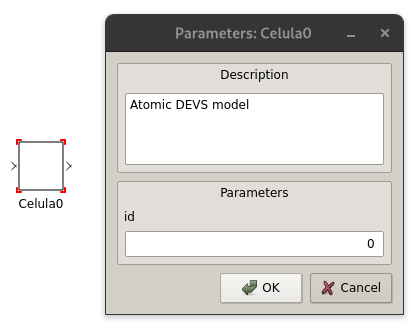
\includegraphics[width=0.5\textwidth]{imagenes/celula.png}
  \caption{Modelo atómico de una célula.}\label{img:celula}
\end{figure}

Una célula se comunica con sus vecinas a través de sus puertos de entrada y salida, como se observa en la figura~\ref{img:conexiones}. Por su puerto de entrada, a lo sumo 8 vecinas le comunican sus cambios de estado (fig.~\ref{img:coneciones_entrada}) y por su puerto de salida les comunica cuando cambia el suyo (fig.~\ref{img:coneciones_salida}).

\begin{figure}[ht]
  \centering
  \begin{subfigure}[b]{0.45\textwidth}
    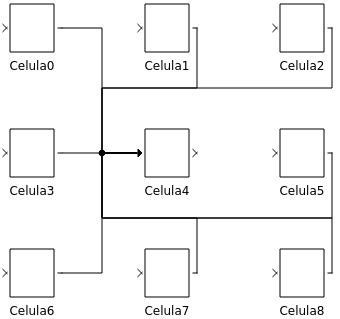
\includegraphics[width=\textwidth]{imagenes/entrada}
    \caption{Conexiones de entrada.}\label{img:coneciones_entrada}
  \end{subfigure}
  \hfill
  \begin{subfigure}[b]{0.45\textwidth}
    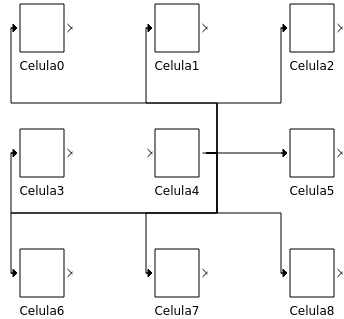
\includegraphics[width=\textwidth]{imagenes/salida}
    \caption{Conexiones de salida.}\label{img:coneciones_salida}
  \end{subfigure}
  \caption{Conexiones de una célula con sus vecinas.}\label{img:conexiones}
\end{figure}

En la figura~\ref{img:tablero} se observa un tablero completo de 4$\times$4 con las conexiones mencionadas anteriormente. Además, cada célula se comunica con un DEVs atómico `Escritor' que se encarga de escribir los resultados de una simulación en un archivo. Es importante establecer el orden de prioridades tal que el Escritor sea el último que realice su transición interna, para que escriba una vez que todas las células le actualizaron su estado.

\begin{figure}[ht]
  \centering
  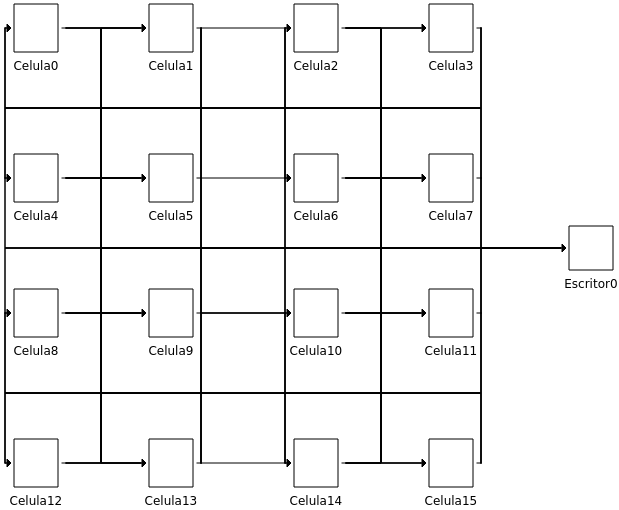
\includegraphics[width=0.75\textwidth]{imagenes/tablero.png}
  \caption{Tablero de 4$\times$4.}\label{img:tablero}
\end{figure}


\subsection{Flujo de evolución}

Cada célula, obtiene su estado inicial, las reglas de supervivencia y nacimiento, y el tiempo entre estados, a través de un archivo de configuración. De la misma manera, el Escritor obtiene el estado inicial del tablero y el tiempo entre estados del mismo archivo.

La simulación consta de dos etapas: una de \textit{Comunicación} y una de \textit{Actualización}. En la primera, cada célula comunica su estado a las vecinas y se escribe en un archivo de salida el estado actual del tablero. En la segunda, cada una actualiza su estado.

Para optimizar este proceso, se lleva una variable $vc \in Bool$ que indica si el vecindario cambió desde la última actualización. Si una célula está en la etapa de Actualización y $vc = F$ entonces no es necesario actualizar su estado, y por lo tanto tampoco es necesario comunicarlo a sus vecinas. Además, si el vecindario sí cambió ($vc = T$) pero el estado resultante es el mismo, tampoco es necesario comunicarlo. En estos casos, la célula no pasa por la etapa de Comunicación hasta que su estado cambie.


\section{Experimentos}


\subsection*{Patrones}

En el juego de la vida de Conway, se pueden observar una amplia variedad de patrones que emergen a medida que las células interactúan entre sí y evolucionan a lo largo de las generaciones. Estos patrones pueden clasificarse en diferentes categorías, que pueden visualizarse en la sección \ref{sec:graficas}:

\begin{itemize}
  \item Patrones estáticos: (fig.~\ref{img:estatico1}-\ref{img:estatico3}) Son patrones que permanecen inalterados a medida que avanzan las generaciones. Estas configuraciones de células forman estructuras estables y no experimentan cambios en su forma o posición. Algunos ejemplos de patrones estáticos son el bloque, que consiste en un grupo de células en forma de cuadrado, y el barco, que consta de una cruz sin centro y una célula adicional en una esquina. También existen otros patrones estáticos como la canoa, la serpiente o la colmena.

  \item Osciladores: (fig.~\ref{img:oscilante1}-\ref{img:oscilante4}) Son patrones que cambian periódicamente entre dos o más estados diferentes. Estos patrones oscilan entre diferentes configuraciones a medida que las generaciones avanzan, pero eventualmente vuelven a su estado inicial. Ejemplos de osciladores incluyen el intermitente, el sapo y el tocino, que alternan entre dos estados en un ciclo constante. También se encuentran otros patrones con un ciclo más largo, como el patrón gema que tiene un ciclo de 5 pasos.

  \item Naves espaciales: (fig.~\ref{img:nave1}-\ref{img:nave4}) Son patrones que se mueven a través de la cuadrícula a medida que evolucionan. Estos patrones exhiben un comportamiento dinámico mientras mantienen su forma relativa. Las células individuales se desplazan y cambian de posición a medida que avanzan las generaciones. Dentro de los ejemplos de naves espaciales se encuentra el planeador, que se desplaza diagonalmente a través de una cuadrícula, así como las naves espaciales que se desplazan en línea recta, como la nave ligera, la nave de peso medio y la nave pesada.
\end{itemize}


\subsection*{Reglas}

Ya vimos que, con las reglas de Conway (23/3), el patrón gema (fig.~\ref{img:oscilante4}) oscila en un ciclo de 5 pasos. En las figuras~\ref{img:sparks}-\ref{img:gema23-36} vemos qué sucede si cambiamos las reglas.


\section{Aplicaciones}

El Juego de la Vida es un modelo que ha sido utilizado para estudiar comportamientos complejos en sistemas dinámicos. A pesar de su simplicidad, exhibe propiedades similares a fenómenos naturales y sociales. Por ejemplo, en biología, ha sido empleado para simular el crecimiento de colonias de células y la propagación de enfermedades. En física, se ha explorado la dinámica de fluidos y el comportamiento de partículas en materiales. Además, ha sido utilizado para modelar fenómenos sociales, como la propagación de altas expectativas y optimismo entre los inversores y participantes del mercado.

Teóricamente, el juego de la vida se considera Turing completo, lo que significa que es capaz de simular cualquier algoritmo computable. Esta afirmación se basa en la posibilidad de crear patrones que simulan puertas lógicas y contadores, lo que permite construir estructuras que realizan cálculos y procesos complejos. Todo esto fue demostrado por Paul Rendell, quien logró construir una máquina de Turing completamente funcional dentro del juego de la vida.

Otros proyectos utilizaron patrones conocidos para recrear sistemas deterministas famosos dentro del juego, como el conocido juego Tetris o incluso replicar el propio juego de la vida dentro de una configuración del mismo. Estos proyectos reflejan aún más la versatilidad y el poder computacional teórico del juego de la vida.


\section{Gráficas de Experimentos}\label{sec:graficas}


% Estaticos

\begin{figure}[h]
  \centering
  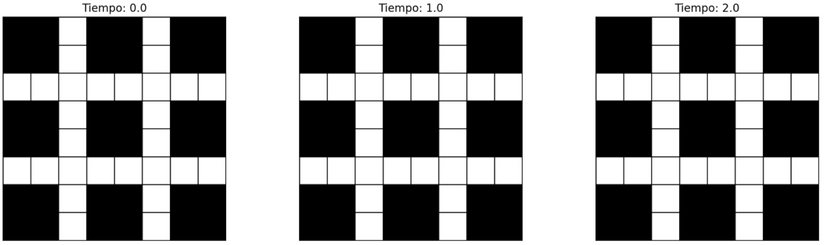
\includegraphics[width=0.8\textwidth]{imagenes/estatico1.png}
  \caption{Ejemplo de patrón bloque replicado en todo el tablero.\label{img:estatico1}}
\end{figure}

\begin{figure}
  \centering
  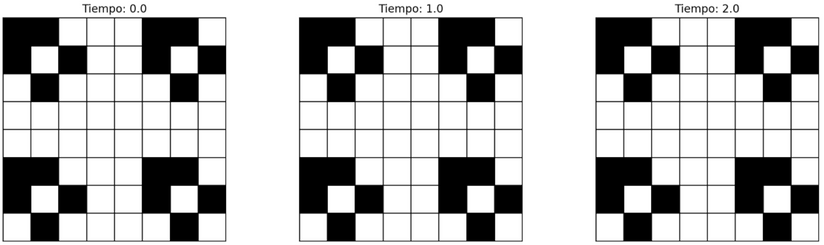
\includegraphics[width=0.8\textwidth]{imagenes/estatico2.png}
  \caption{Ejemplo de patrón bote replicado cuatro veces.\label{img:estatico2}}
\end{figure}

\begin{figure}
  \centering
  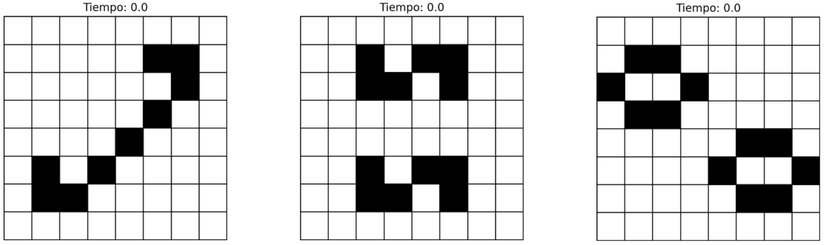
\includegraphics[width=0.8\textwidth]{imagenes/estatico3.png}
  \caption{Patrones canoa, serpiente y colmena\label{img:estatico3}}
\end{figure}


% Osciladores

\begin{figure}
  \centering
  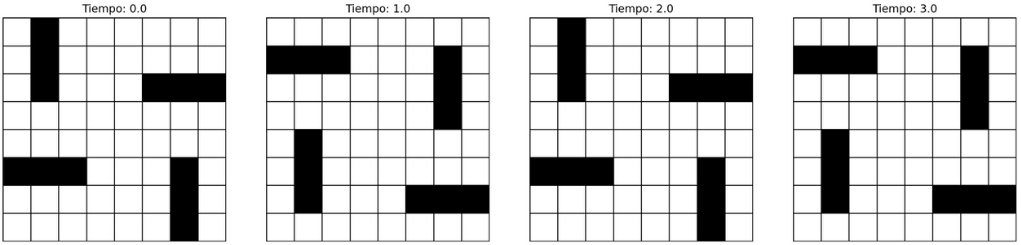
\includegraphics[width=0.8\textwidth]{imagenes/oscilante1.png}
  \caption{Ejemplo de patrón intermitente.\label{img:oscilante1}}
\end{figure}

\begin{figure}
  \centering
  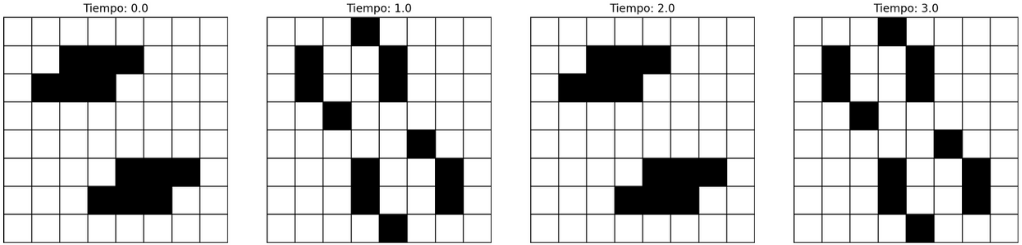
\includegraphics[width=0.8\textwidth]{imagenes/oscilante2.png}
  \caption{Ejemplo de patrón sapo.\label{img:oscilante2}}
\end{figure}

\begin{figure}
  \centering
  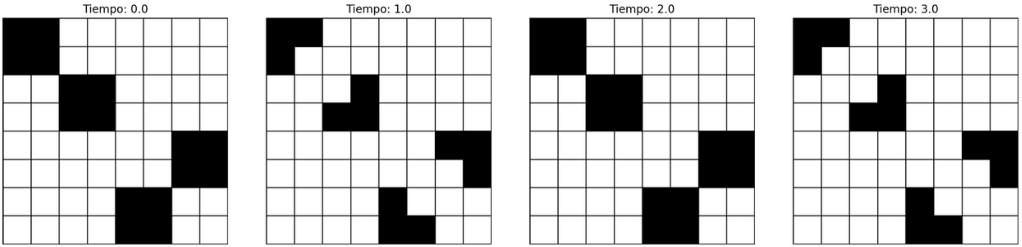
\includegraphics[width=0.8\textwidth]{imagenes/oscilante3.png}
  \caption{Ejemplo de patrón tocino.\label{img:oscilante3}}
\end{figure}

\begin{figure}
  \centering
  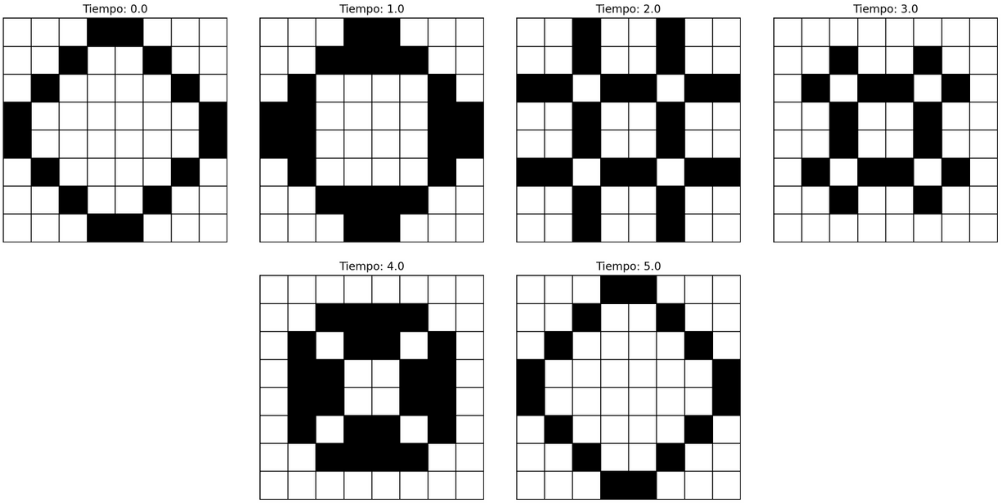
\includegraphics[width=0.8\textwidth]{imagenes/oscilante4.png}
  \caption{Ejemplo de patrón gema.\label{img:oscilante4}}
\end{figure}


% Naves espaciales

\begin{figure}
  \centering
  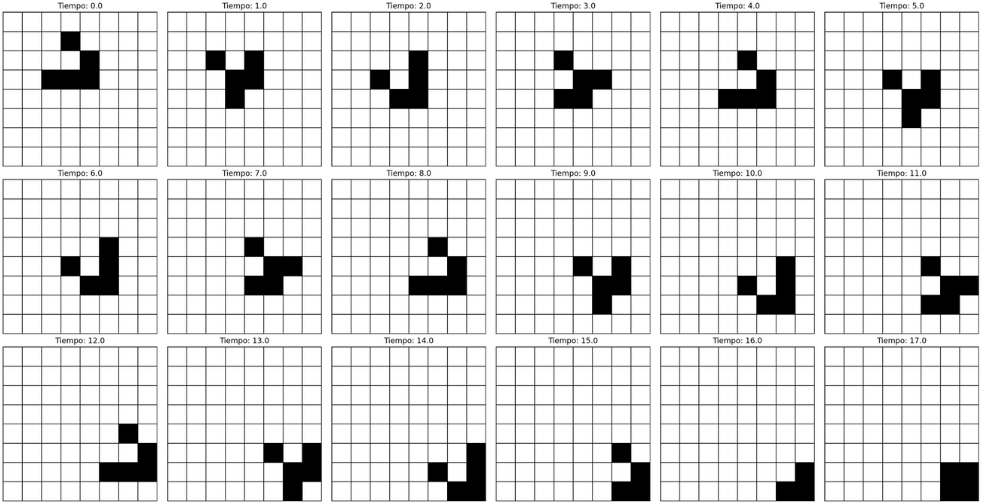
\includegraphics[width=0.8\textwidth]{imagenes/nave1.png}
  \caption{Patrón Planeador. Es importante tener en cuenta que el patrón del planeador se estabiliza en un patrón bloque cuando alcanza los límites de una cuadrícula finita, lo cual no ocurriría en una cuadrícula infinita. De manera similar, en el caso de las naves espaciales, cuando estas alcanzan la pared, el patrón se rompe. Sin embargo, en una cuadrícula infinita, estas naves seguirían desplazándose hacia la derecha indefinidamente.\label{img:nave1}}
\end{figure}

\begin{figure}
  \centering
  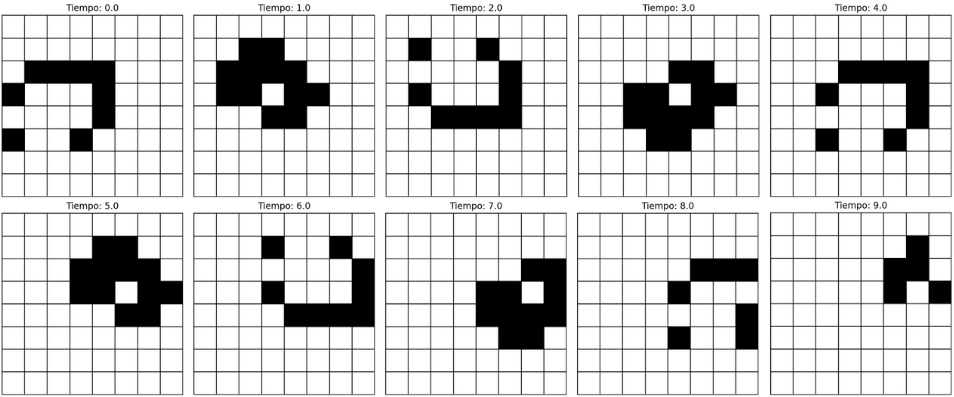
\includegraphics[width=0.8\textwidth]{imagenes/nave2.png}
  \caption{Patrón Nave ligera.\label{img:nave2}}
\end{figure}

\begin{figure}
  \centering
  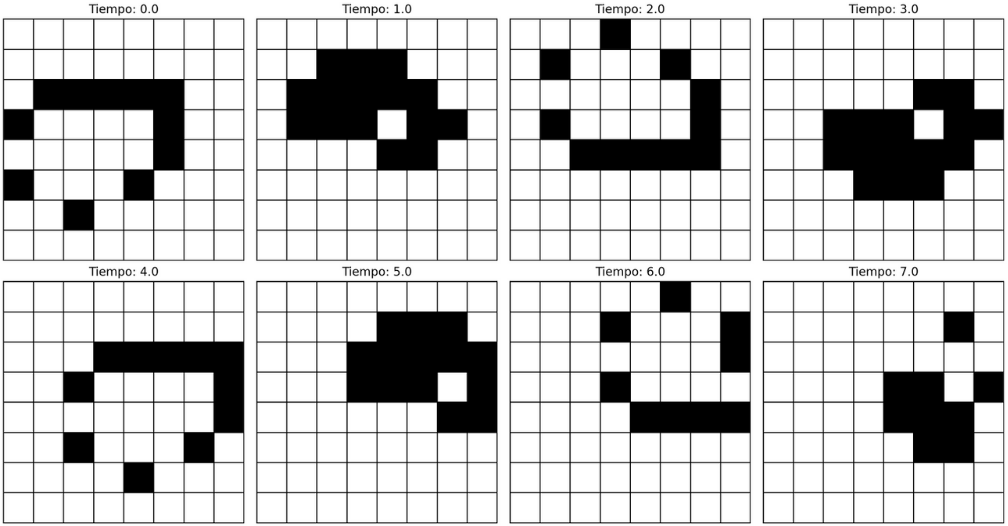
\includegraphics[width=0.8\textwidth]{imagenes/nave3.png}
  \caption{Patrón Nave de peso medio.\label{img:nave3}}
\end{figure}

\begin{figure}
  \centering
  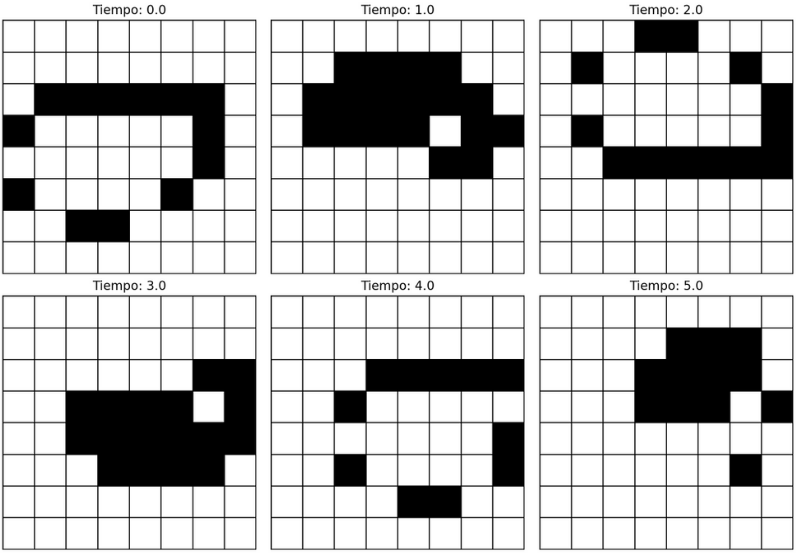
\includegraphics[width=0.8\textwidth]{imagenes/nave4.png}
  \caption{Patrón Nave pesada.\label{img:nave4}}
\end{figure}

\begin{figure}
  \centering
  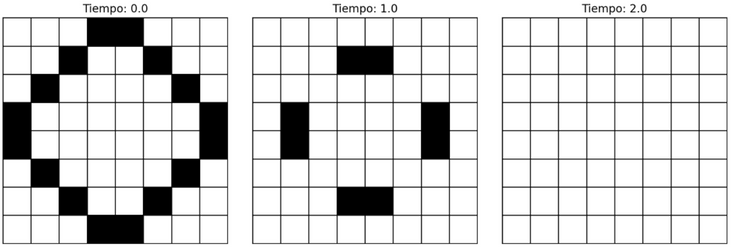
\includegraphics[width=0.8\textwidth]{imagenes/sparks.png}
  \caption{Patrón gema con regla /3 ``Sparks''. Las células se extinguen rápidamente debido a la falta de reglas de supervivencia.\label{img:sparks}}
\end{figure}

\begin{figure}
  \centering
  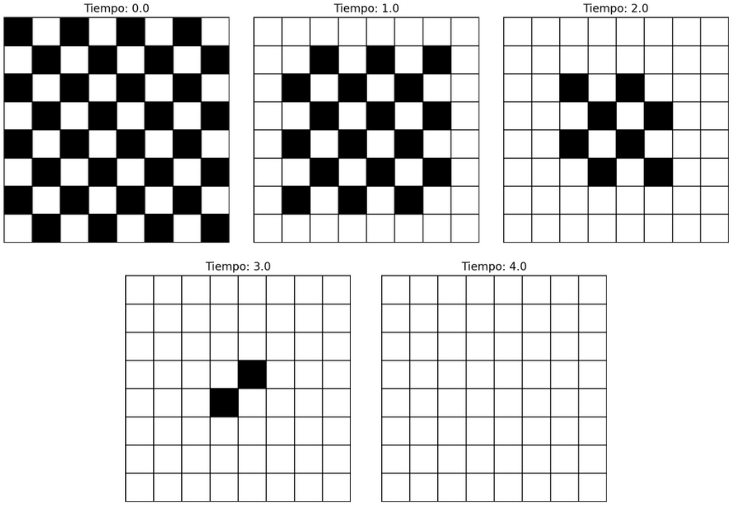
\includegraphics[width=0.8\textwidth]{imagenes/sparks2.png}
  \caption{Secuencia donde se extinguen las células con reglas ``\_/4''. Hay una gran cantidad de células vivas que se extinguen a medida que avanzan las generaciones.\label{img:sparks2}}
\end{figure}

\begin{figure}
  \centering
  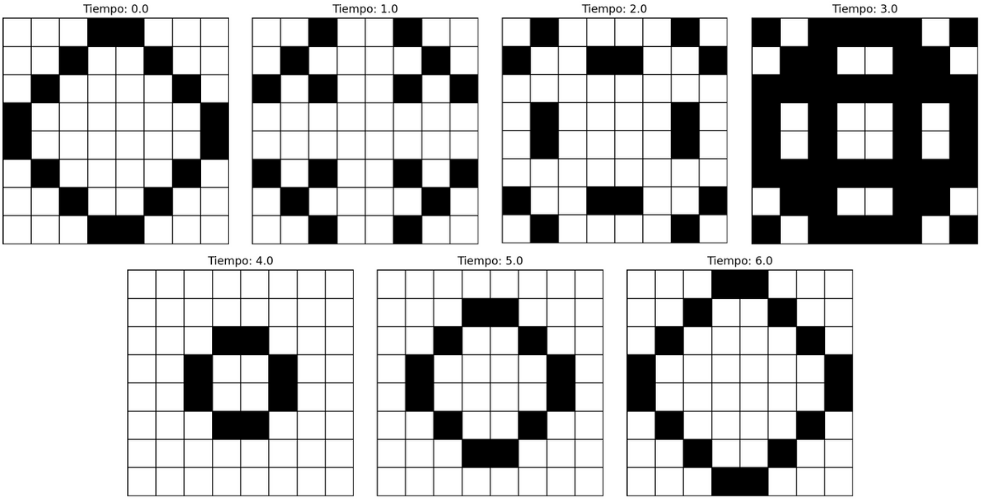
\includegraphics[width=0.8\textwidth]{imagenes/gema4-2.png}
  \caption{Patrón gema con regla 4/2. Con estas reglas se puede ver que el ciclo se extendió de 5 a 6 pasos.\label{img:gema4-2}}
\end{figure}

\begin{figure}
  \centering
  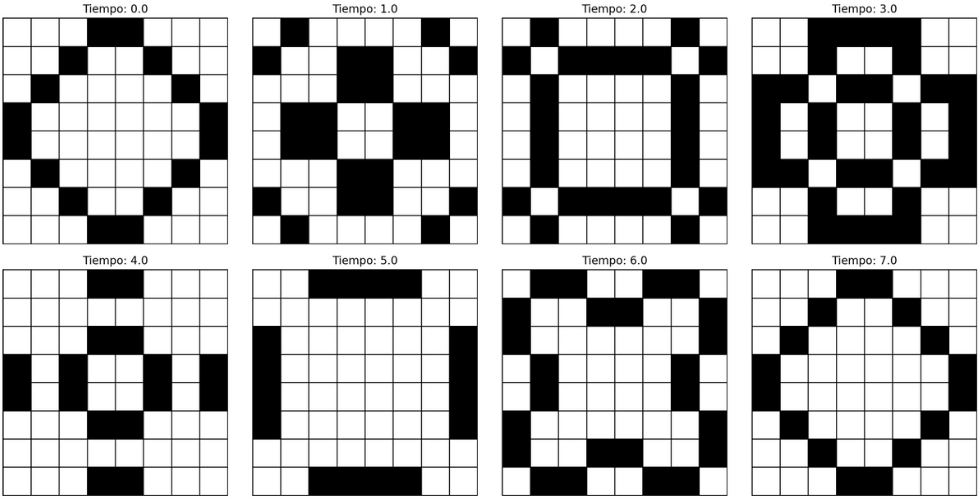
\includegraphics[width=0.8\textwidth]{imagenes/gema1357-1357.png}
  \caption{Patrón gema con regla 1357/1357 ``Breeder''. Con estas reglas se puede ver que el ciclo se ha prolongado de 5 a 7 pasos.\label{img:gema1357-1357}}
\end{figure}

\begin{figure}
  \centering
  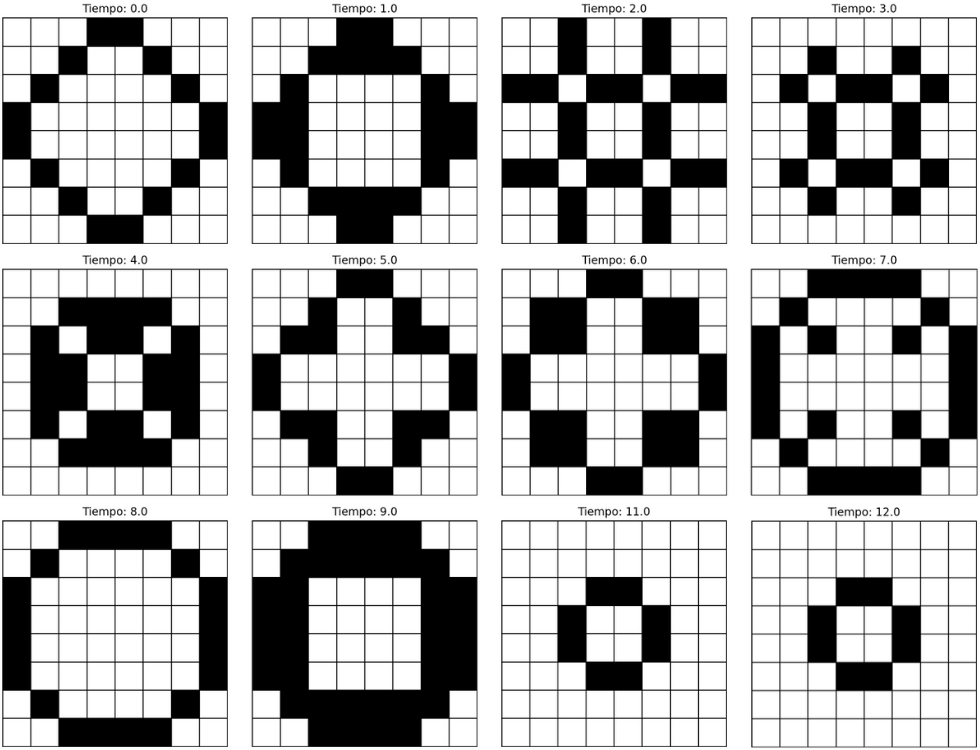
\includegraphics[width=0.8\textwidth]{imagenes/gema23-36.png}
  \caption{Patrón gema con regla 23/36 ``HighLife''. Esta configuración es similar al juego de la vida de Conway, pero con la adición de una nueva regla que permite el nacimiento de células cuando tienen 6 vecinos vivos. Se puede ver que las primeras cuatro generaciones son idénticas al patrón gema con las reglas de conway, pero que en el quinto paso se rompe el ciclo original por la adición de la regla anteriormente mencionada. En este caso, el patrón deja de oscilar y se estabiliza en el paso 11.\label{img:gema23-36}}
\end{figure}

\end{document}
